\chapter{The Story}

First, sir,” said Caderousse, “you must make me a promise.”

“What is that?” inquired the abbé.

“Why, if you ever make use of the details I am about to give you, that
you will never let anyone know that it was I who supplied them; for the
persons of whom I am about to talk are rich and powerful, and if they
only laid the tips of their fingers on me, I should break to pieces
like glass.”

“Make yourself easy, my friend,” replied the abbé. “I am a priest, and
confessions die in my breast. Recollect, our only desire is to carry
out, in a fitting manner, the last wishes of our friend. Speak, then,
without reserve, as without hatred; tell the truth, the whole truth; I
do not know, never may know, the persons of whom you are about to
speak; besides, I am an Italian, and not a Frenchman, and belong to
God, and not to man, and I shall shortly retire to my convent, which I
have only quitted to fulfil the last wishes of a dying man.”

This positive assurance seemed to give Caderousse a little courage.

“Well, then, under these circumstances,” said Caderousse, “I will, I
even believe I ought to undeceive you as to the friendship which poor
Edmond thought so sincere and unquestionable.”

“Begin with his father, if you please.” said the abbé; “Edmond talked
to me a great deal about the old man for whom he had the deepest love.”

“The history is a sad one, sir,” said Caderousse, shaking his head;
“perhaps you know all the earlier part of it?”

“Yes.” answered the abbé; “Edmond related to me everything until the
moment when he was arrested in a small cabaret close to Marseilles.”

“At La Réserve! Oh, yes; I can see it all before me this moment.”

“Was it not his betrothal feast?”

“It was and the feast that began so gayly had a very sorrowful ending;
a police commissary, followed by four soldiers, entered, and Dantès was
arrested.”

“Yes, and up to this point I know all,” said the priest. “Dantès
himself only knew that which personally concerned him, for he never
beheld again the five persons I have named to you, or heard mention of
anyone of them.”

“Well, when Dantès was arrested, Monsieur Morrel hastened to obtain the
particulars, and they were very sad. The old man returned alone to his
home, folded up his wedding suit with tears in his eyes, and paced up
and down his chamber the whole day, and would not go to bed at all, for
I was underneath him and heard him walking the whole night; and for
myself, I assure you I could not sleep either, for the grief of the
poor father gave me great uneasiness, and every step he took went to my
heart as really as if his foot had pressed against my breast.

“The next day Mercédès came to implore the protection of M. de
Villefort; she did not obtain it, however, and went to visit the old
man; when she saw him so miserable and heart-broken, having passed a
sleepless night, and not touched food since the previous day, she
wished him to go with her that she might take care of him; but the old
man would not consent. ‘No,’ was the old man’s reply, ‘I will not leave
this house, for my poor dear boy loves me better than anything in the
world; and if he gets out of prison he will come and see me the first
thing, and what would he think if I did not wait here for him?’ I heard
all this from the window, for I was anxious that Mercédès should
persuade the old man to accompany her, for his footsteps over my head
night and day did not leave me a moment’s repose.”

“But did you not go upstairs and try to console the poor old man?”
asked the abbé.

“Ah, sir,” replied Caderousse, “we cannot console those who will not be
consoled, and he was one of these; besides, I know not why, but he
seemed to dislike seeing me. One night, however, I heard his sobs, and
I could not resist my desire to go up to him, but when I reached his
door he was no longer weeping but praying. I cannot now repeat to you,
sir, all the eloquent words and imploring language he made use of; it
was more than piety, it was more than grief, and I, who am no canter,
and hate the Jesuits, said then to myself, ‘It is really well, and I am
very glad that I have not any children; for if I were a father and felt
such excessive grief as the old man does, and did not find in my memory
or heart all he is now saying, I should throw myself into the sea at
once, for I could not bear it.’”

“Poor father!” murmured the priest.

“From day to day he lived on alone, and more and more solitary. M.
Morrel and Mercédès came to see him, but his door was closed; and,
although I was certain he was at home, he would not make any answer.
One day, when, contrary to his custom, he had admitted Mercédès, and
the poor girl, in spite of her own grief and despair, endeavored to
console him, he said to her,—‘Be assured, my dear daughter, he is dead;
and instead of expecting him, it is he who is awaiting us; I am quite
happy, for I am the oldest, and of course shall see him first.’

“However well disposed a person may be, why, you see we leave off after
a time seeing persons who are in sorrow, they make one melancholy; and
so at last old Dantès was left all to himself, and I only saw from time
to time strangers go up to him and come down again with some bundle
they tried to hide; but I guessed what these bundles were, and that he
sold by degrees what he had to pay for his subsistence. At length the
poor old fellow reached the end of all he had; he owed three quarters’
rent, and they threatened to turn him out; he begged for another week,
which was granted to him. I know this, because the landlord came into
my apartment when he left his.

“For the first three days I heard him walking about as usual, but, on
the fourth I heard nothing. I then resolved to go up to him at all
risks. The door was closed, but I looked through the keyhole, and saw
him so pale and haggard, that believing him very ill, I went and told
M. Morrel and then ran on to Mercédès. They both came immediately, M.
Morrel bringing a doctor, and the doctor said it was inflammation of
the bowels, and ordered him a limited diet. I was there, too, and I
never shall forget the old man’s smile at this prescription.

“From that time he received all who came; he had an excuse for not
eating any more; the doctor had put him on a diet.”

The abbé uttered a kind of groan.

“The story interests you, does it not, sir?” inquired Caderousse.

“Yes,” replied the abbé, “it is very affecting.”

“Mercédès came again, and she found him so altered that she was even
more anxious than before to have him taken to her own home. This was M.
Morrel’s wish also, who would fain have conveyed the old man against
his consent; but the old man resisted, and cried so that they were
actually frightened. Mercédès remained, therefore, by his bedside, and
M. Morrel went away, making a sign to the Catalan that he had left his
purse on the chimney-piece; but, availing himself of the doctor’s
order, the old man would not take any sustenance; at length (after nine
days of despair and fasting), the old man died, cursing those who had
caused his misery, and saying to Mercédès, ‘If you ever see my Edmond
again, tell him I die blessing him.’”

The abbé rose from his chair, made two turns round the chamber, and
pressed his trembling hand against his parched throat.

“And you believe he died——”

“Of hunger, sir, of hunger,” said Caderousse. “I am as certain of it as
that we two are Christians.”

The abbé, with a shaking hand, seized a glass of water that was
standing by him half-full, swallowed it at one gulp, and then resumed
his seat, with red eyes and pale cheeks.

“This was, indeed, a horrid event,” said he in a hoarse voice.

“The more so, sir, as it was men’s and not God’s doing.”

“Tell me of those men,” said the abbé, “and remember too,” he added in
an almost menacing tone, “you have promised to tell me everything. Tell
me, therefore, who are these men who killed the son with despair, and
the father with famine?”

“Two men jealous of him, sir; one from love, and the other from
ambition,—Fernand and Danglars.”

“How was this jealousy manifested? Speak on.”

“They denounced Edmond as a Bonapartist agent.”

“Which of the two denounced him? Which was the real delinquent?”

“Both, sir; one with a letter, and the other put it in the post.”

“And where was this letter written?”

“At La Réserve, the day before the betrothal feast.”

“’Twas so, then—’twas so, then,” murmured the abbé. “Oh, Faria, Faria,
how well did you judge men and things!”

“What did you please to say, sir?” asked Caderousse.

“Nothing, nothing,” replied the priest; “go on.”

“It was Danglars who wrote the denunciation with his left hand, that
his writing might not be recognized, and Fernand who put it in the
post.”

“But,” exclaimed the abbé suddenly, “you were there yourself.”

“I!” said Caderousse, astonished; “who told you I was there?”

The abbé saw he had overshot the mark, and he added quickly,—“No one;
but in order to have known everything so well, you must have been an
eye-witness.”

“True, true!” said Caderousse in a choking voice, “I was there.”

“And did you not remonstrate against such infamy?” asked the abbé; “if
not, you were an accomplice.”

“Sir,” replied Caderousse, “they had made me drink to such an excess
that I nearly lost all perception. I had only an indistinct
understanding of what was passing around me. I said all that a man in
such a state could say; but they both assured me that it was a jest
they were carrying on, and perfectly harmless.”

“Next day—next day, sir, you must have seen plain enough what they had
been doing, yet you said nothing, though you were present when Dantès
was arrested.”

“Yes, sir, I was there, and very anxious to speak; but Danglars
restrained me. ‘If he should really be guilty,’ said he, ‘and did
really put in to the Island of Elba; if he is really charged with a
letter for the Bonapartist committee at Paris, and if they find this
letter upon him, those who have supported him will pass for his
accomplices.’ I confess I had my fears, in the state in which politics
then were, and I held my tongue. It was cowardly, I confess, but it was
not criminal.”

\begin{figure}[ht]
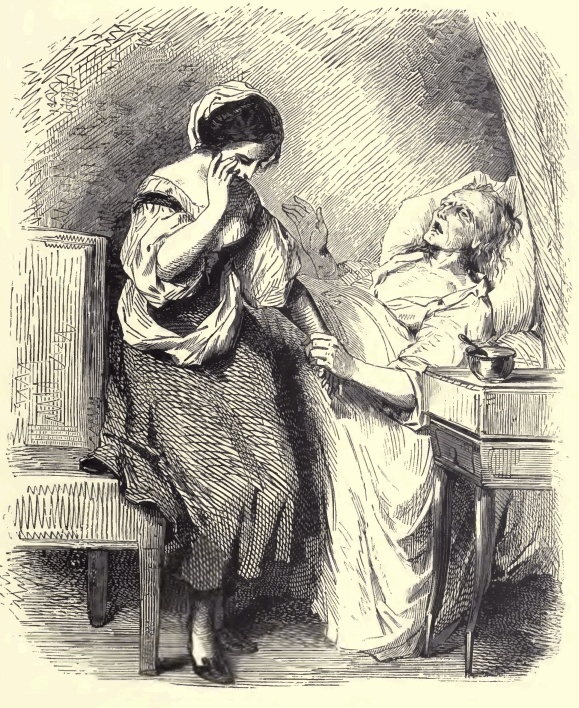
\includegraphics[width=\textwidth]{0341m.jpg}
\end{figure}

“I understand—you allowed matters to take their course, that was all.”

“Yes, sir,” answered Caderousse; “and remorse preys on me night and
day. I often ask pardon of God, I swear to you, because this action,
the only one with which I have seriously to reproach myself in all my
life, is no doubt the cause of my abject condition. I am expiating a
moment of selfishness, and so I always say to La Carconte, when she
complains, ‘Hold your tongue, woman; it is the will of God.’” And
Caderousse bowed his head with every sign of real repentance.

“Well, sir,” said the abbé, “you have spoken unreservedly; and thus to
accuse yourself is to deserve pardon.”

“Unfortunately, Edmond is dead, and has not pardoned me.”

“He did not know,” said the abbé.

“But he knows it all now,” interrupted Caderousse; “they say the dead
know everything.”

There was a brief silence; the abbé rose and paced up and down
pensively, and then resumed his seat.

“You have two or three times mentioned a M. Morrel,” he said; “who was
he?”

“The owner of the \textit{Pharaon} and patron of Dantès.”

“And what part did he play in this sad drama?” inquired the abbé.

“The part of an honest man, full of courage and real regard. Twenty
times he interceded for Edmond. When the emperor returned, he wrote,
implored, threatened, and so energetically, that on the second
restoration he was persecuted as a Bonapartist. Ten times, as I told
you, he came to see Dantès’ father, and offered to receive him in his
own house; and the night or two before his death, as I have already
said, he left his purse on the mantelpiece, with which they paid the
old man’s debts, and buried him decently; and so Edmond’s father died,
as he had lived, without doing harm to anyone. I have the purse still
by me—a large one, made of red silk.”

“And,” asked the abbé, “is M. Morrel still alive?”

“Yes,” replied Caderousse.

“In that case,” replied the abbé, “he should be a man blessed of God,
rich, happy.”

Caderousse smiled bitterly. “Yes, happy as myself,” said he.

“What! M. Morrel unhappy?” exclaimed the abbé.

“He is reduced almost to the last extremity—nay, he is almost at the
point of dishonor.”

“How?”

“Yes,” continued Caderousse, “so it is; after five-and-twenty years of
labor, after having acquired a most honorable name in the trade of
Marseilles, M. Morrel is utterly ruined; he has lost five ships in two
years, has suffered by the bankruptcy of three large houses, and his
only hope now is in that very \textit{Pharaon} which poor Dantès commanded,
and which is expected from the Indies with a cargo of cochineal and
indigo. If this ship founders, like the others, he is a ruined man.”

“And has the unfortunate man wife or children?” inquired the abbé.

“Yes, he has a wife, who through everything has behaved like an angel;
he has a daughter, who was about to marry the man she loved, but whose
family now will not allow him to wed the daughter of a ruined man; he
has, besides, a son, a lieutenant in the army; and, as you may suppose,
all this, instead of lessening, only augments his sorrows. If he were
alone in the world he would blow out his brains, and there would be an
end.”

“Horrible!” ejaculated the priest.

“And it is thus heaven recompenses virtue, sir,” added Caderousse. “You
see, I, who never did a bad action but that I have told you of—am in
destitution, with my poor wife dying of fever before my very eyes, and
I unable to do anything in the world for her; I shall die of hunger, as
old Dantès did, while Fernand and Danglars are rolling in wealth.”

“How is that?”

“Because their deeds have brought them good fortune, while honest men
have been reduced to misery.”

“What has become of Danglars, the instigator, and therefore the most
guilty?”

“What has become of him? Why, he left Marseilles, and was taken, on the
recommendation of M. Morrel, who did not know his crime, as cashier
into a Spanish bank. During the war with Spain he was employed in the
commissariat of the French army, and made a fortune; then with that
money he speculated in the funds, and trebled or quadrupled his
capital; and, having first married his banker’s daughter, who left him
a widower, he has married a second time, a widow, a Madame de Nargonne,
daughter of M. de Servieux, the king’s chamberlain, who is in high
favor at court. He is a millionaire, and they have made him a baron,
and now he is the Baron Danglars, with a fine residence in the Rue du
Mont-Blanc, with ten horses in his stables, six footmen in his
antechamber, and I know not how many millions in his strongbox.”

“Ah!” said the abbé, in a peculiar tone, “he is happy.”

“Happy? Who can answer for that? Happiness or unhappiness is the secret
known but to one’s self and the walls—walls have ears but no tongue;
but if a large fortune produces happiness, Danglars is happy.”

“And Fernand?”

“Fernand? Why, much the same story.”

“But how could a poor Catalan fisher-boy, without education or
resources, make a fortune? I confess this staggers me.”

“And it has staggered everybody. There must have been in his life some
strange secret that no one knows.”

“But, then, by what visible steps has he attained this high fortune or
high position?”

“Both, sir—he has both fortune and position—both.”

“This must be impossible!”

“It would seem so; but listen, and you will understand. Some days
before the return of the emperor, Fernand was drafted. The Bourbons
left him quietly enough at the Catalans, but Napoleon returned, a
special levy was made, and Fernand was compelled to join. I went too;
but as I was older than Fernand, and had just married my poor wife, I
was only sent to the coast. Fernand was enrolled in the active army,
went to the frontier with his regiment, and was at the battle of Ligny.
The night after that battle he was sentry at the door of a general who
carried on a secret correspondence with the enemy. That same night the
general was to go over to the English. He proposed to Fernand to
accompany him; Fernand agreed to do so, deserted his post, and followed
the general.

“Fernand would have been court-martialed if Napoleon had remained on
the throne, but his action was rewarded by the Bourbons. He returned to
France with the epaulet of sub-lieutenant, and as the protection of the
general, who is in the highest favor, was accorded to him, he was a
captain in 1823, during the Spanish war—that is to say, at the time
when Danglars made his early speculations. Fernand was a Spaniard, and
being sent to Spain to ascertain the feeling of his fellow-countrymen,
found Danglars there, got on very intimate terms with him, won over the
support of the royalists at the capital and in the provinces, received
promises and made pledges on his own part, guided his regiment by paths
known to himself alone through the mountain gorges which were held by
the royalists, and, in fact, rendered such services in this brief
campaign that, after the taking of Trocadero, he was made colonel, and
received the title of count and the cross of an officer of the Legion
of Honor.”

“Destiny! destiny!” murmured the abbé.

“Yes, but listen: this was not all. The war with Spain being ended,
Fernand’s career was checked by the long peace which seemed likely to
endure throughout Europe. Greece only had risen against Turkey, and had
begun her war of independence; all eyes were turned towards Athens—it
was the fashion to pity and support the Greeks. The French government,
without protecting them openly, as you know, gave countenance to
volunteer assistance. Fernand sought and obtained leave to go and serve
in Greece, still having his name kept on the army roll.

\begin{figure}[ht]
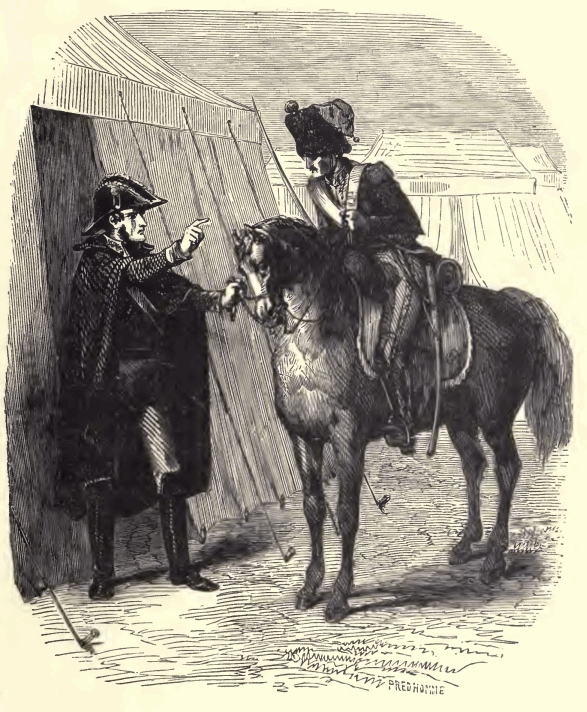
\includegraphics[width=\textwidth]{0345m.jpg}
\end{figure}

Some time after, it was stated that the Comte de Morcerf (this was the
name he bore) had entered the service of Ali Pasha with the rank of
instructor-general. Ali Pasha was killed, as you know, but before he
died he recompensed the services of Fernand by leaving him a
considerable sum, with which he returned to France, when he was
gazetted lieutenant-general.”

“So that now——?” inquired the abbé.

“So that now,” continued Caderousse, “he owns a magnificent house—No.
27, Rue du Helder, Paris.”

The abbé opened his mouth, hesitated for a moment, then, making an
effort at self-control, he said, “And Mercédès—they tell me that she
has disappeared?”

“Disappeared,” said Caderousse, “yes, as the sun disappears, to rise
the next day with still more splendor.”

“Has she made a fortune also?” inquired the abbé, with an ironical
smile.

“Mercédès is at this moment one of the greatest ladies in Paris,”
replied Caderousse.

“Go on,” said the abbé; “it seems as if I were listening to the story
of a dream. But I have seen things so extraordinary, that what you tell
me seems less astonishing than it otherwise might.”

“Mercédès was at first in the deepest despair at the blow which
deprived her of Edmond. I have told you of her attempts to propitiate
M. de Villefort, her devotion to the elder Dantès. In the midst of her
despair, a new affliction overtook her. This was the departure of
Fernand—of Fernand, whose crime she did not know, and whom she regarded
as her brother. Fernand went, and Mercédès remained alone.

“Three months passed and still she wept—no news of Edmond, no news of
Fernand, no companionship save that of an old man who was dying with
despair. One evening, after a day of accustomed vigil at the angle of
two roads leading to Marseilles from the Catalans, she returned to her
home more depressed than ever. Suddenly she heard a step she knew,
turned anxiously around, the door opened, and Fernand, dressed in the
uniform of a sub-lieutenant, stood before her.

“It was not the one she wished for most, but it seemed as if a part of
her past life had returned to her.

“Mercédès seized Fernand’s hands with a transport which he took for
love, but which was only joy at being no longer alone in the world, and
seeing at last a friend, after long hours of solitary sorrow. And then,
it must be confessed, Fernand had never been hated—he was only not
precisely loved. Another possessed all Mercédès’ heart; that other was
absent, had disappeared, perhaps was dead. At this last thought
Mercédès burst into a flood of tears, and wrung her hands in agony; but
the thought, which she had always repelled before when it was suggested
to her by another, came now in full force upon her mind; and then, too,
old Dantès incessantly said to her, ‘Our Edmond is dead; if he were
not, he would return to us.’

“The old man died, as I have told you; had he lived, Mercédès,
perchance, had not become the wife of another, for he would have been
there to reproach her infidelity. Fernand saw this, and when he learned
of the old man’s death he returned. He was now a lieutenant. At his
first coming he had not said a word of love to Mercédès; at the second
he reminded her that he loved her.

“Mercédès begged for six months more in which to await and mourn for
Edmond.”

“So that,” said the abbé, with a bitter smile, “that makes eighteen
months in all. What more could the most devoted lover desire?” Then he
murmured the words of the English poet, “‘Frailty, thy name is woman.’”

“Six months afterwards,” continued Caderousse, “the marriage took place
in the church of Accoules.”

“The very church in which she was to have married Edmond,” murmured the
priest; “there was only a change of bridegrooms.”

“Well, Mercédès was married,” proceeded Caderousse; “but although in
the eyes of the world she appeared calm, she nearly fainted as she
passed La Réserve, where, eighteen months before, the betrothal had
been celebrated with him whom she might have known she still loved, had
she looked to the bottom of her heart. Fernand, more happy, but not
more at his ease—for I saw at this time he was in constant dread of
Edmond’s return—Fernand was very anxious to get his wife away, and to
depart himself. There were too many unpleasant possibilities associated
with the Catalans, and eight days after the wedding they left
Marseilles.”

“Did you ever see Mercédès again?” inquired the priest.

“Yes, during the Spanish war, at Perpignan, where Fernand had left her;
she was attending to the education of her son.”

The abbé started. “Her son?” said he.

“Yes,” replied Caderousse, “little Albert.”

“But, then, to be able to instruct her child,” continued the abbé, “she
must have received an education herself. I understood from Edmond that
she was the daughter of a simple fisherman, beautiful but uneducated.”

“Oh,” replied Caderousse, “did he know so little of his lovely
betrothed? Mercédès might have been a queen, sir, if the crown were to
be placed on the heads of the loveliest and most intelligent. Fernand’s
fortune was already waxing great, and she developed with his growing
fortune. She learned drawing, music—everything. Besides, I believe,
between ourselves, she did this in order to distract her mind, that she
might forget; and she only filled her head in order to alleviate the
weight on her heart. But now her position in life is assured,”
continued Caderousse; “no doubt fortune and honors have comforted her;
she is rich, a countess, and yet——”

Caderousse paused.

“And yet what?” asked the abbé.

“Yet, I am sure, she is not happy,” said Caderousse.

“What makes you believe this?”

“Why, when I found myself utterly destitute, I thought my old friends
would, perhaps, assist me. So I went to Danglars, who would not even
receive me. I called on Fernand, who sent me a hundred francs by his
valet-de-chambre.”

“Then you did not see either of them?”

“No, but Madame de Morcerf saw me.”

“How was that?”

“As I went away a purse fell at my feet—it contained five-and-twenty
louis; I raised my head quickly, and saw Mercédès, who at once shut the
blind.”

“And M. de Villefort?” asked the abbé.

“Oh, he never was a friend of mine, I did not know him, and I had
nothing to ask of him.”

“Do you not know what became of him, and the share he had in Edmond’s
misfortunes?”

“No; I only know that some time after Edmond’s arrest, he married
Mademoiselle de Saint-Méran, and soon after left Marseilles; no doubt
he has been as lucky as the rest; no doubt he is as rich as Danglars,
as high in station as Fernand. I only, as you see, have remained poor,
wretched, and forgotten.”

“You are mistaken, my friend,” replied the abbé; “God may seem
sometimes to forget for a time, while his justice reposes, but there
always comes a moment when he remembers—and behold—a proof!”

As he spoke, the abbé took the diamond from his pocket, and giving it
to Caderousse, said, “Here, my friend, take this diamond, it is yours.”

“What, for me only?” cried Caderousse, “ah, sir, do not jest with me!”

“This diamond was to have been shared among his friends. Edmond had one
friend only, and thus it cannot be divided. Take the diamond, then, and
sell it; it is worth fifty thousand francs, and I repeat my wish that
this sum may suffice to release you from your wretchedness.”

\begin{figure}[ht]
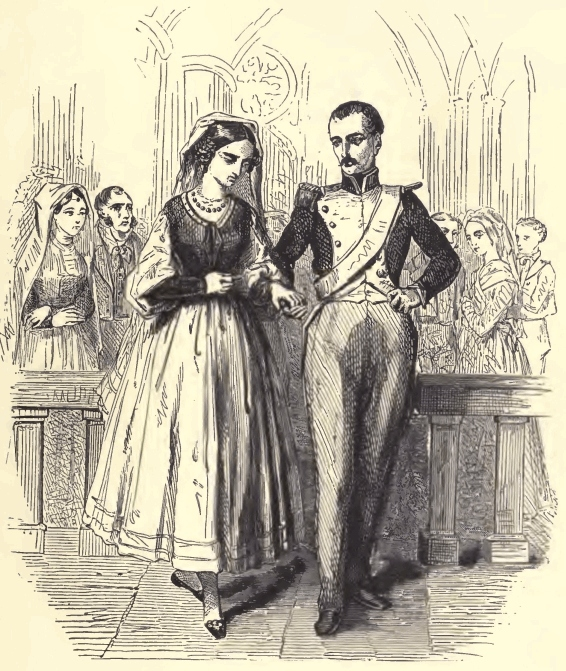
\includegraphics[width=\textwidth]{0351m.jpg}
\end{figure}

“Oh, sir,” said Caderousse, putting out one hand timidly, and with the
other wiping away the perspiration which bedewed his brow,—“Oh, sir, do
not make a jest of the happiness or despair of a man.”

“I know what happiness and what despair are, and I never make a jest of
such feelings. Take it, then, but in exchange——”

Caderousse, who touched the diamond, withdrew his hand.

The abbé smiled.

“In exchange,” he continued, “give me the red silk purse that M. Morrel
left on old Dantès’ chimney-piece, and which you tell me is still in
your hands.”

Caderousse, more and more astonished, went toward a large oaken
cupboard, opened it, and gave the abbé a long purse of faded red silk,
round which were two copper runners that had once been gilt. The abbé
took it, and in return gave Caderousse the diamond.

“Oh, you are a man of God, sir,” cried Caderousse; “for no one knew
that Edmond had given you this diamond, and you might have kept it.”

“Which,” said the abbé to himself, “you would have done.” The abbé
rose, took his hat and gloves. “Well,” he said, “all you have told me
is perfectly true, then, and I may believe it in every particular.”

“See, sir,” replied Caderousse, “in this corner is a crucifix in holy
wood—here on this shelf is my wife’s testament; open this book, and I
will swear upon it with my hand on the crucifix. I will swear to you by
my soul’s salvation, my faith as a Christian, I have told everything to
you as it occurred, and as the recording angel will tell it to the ear
of God at the day of the last judgment!”

“’Tis well,” said the abbé, convinced by his manner and tone that
Caderousse spoke the truth. “’Tis well, and may this money profit you!
Adieu; I go far from men who thus so bitterly injure each other.”

The abbé with difficulty got away from the enthusiastic thanks of
Caderousse, opened the door himself, got out and mounted his horse,
once more saluted the innkeeper, who kept uttering his loud farewells,
and then returned by the road he had travelled in coming.

When Caderousse turned around, he saw behind him La Carconte, paler and
trembling more than ever.

“Is, then, all that I have heard really true?” she inquired.

“What? That he has given the diamond to us only?” inquired Caderousse,
half bewildered with joy; “yes, nothing more true! See, here it is.”

The woman gazed at it a moment, and then said, in a gloomy voice,
“Suppose it’s false?”

Caderousse started and turned pale.

“False!” he muttered. “False! Why should that man give me a false
diamond?”

\begin{figure}[ht]
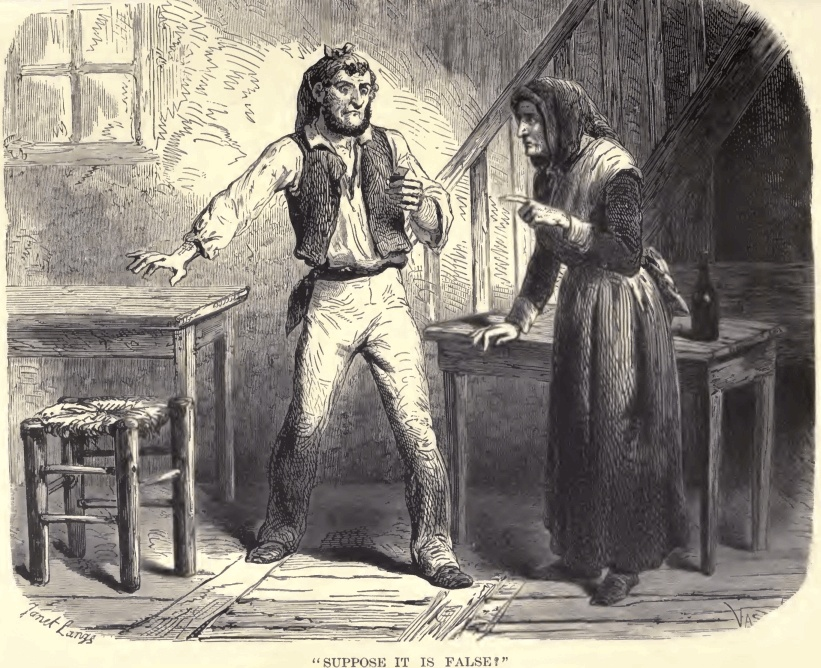
\includegraphics[width=\textwidth]{0349m.jpg}
\end{figure}

“To get your secret without paying for it, you blockhead!”

Caderousse remained for a moment aghast under the weight of such an
idea.

“Oh!” he said, taking up his hat, which he placed on the red
handkerchief tied round his head, “we will soon find out.”

“In what way?”

“Why, the fair is on at Beaucaire, there are always jewellers from
Paris there, and I will show it to them. Look after the house, wife,
and I shall be back in two hours,” and Caderousse left the house in
haste, and ran rapidly in the direction opposite to that which the
priest had taken.

“Fifty thousand francs!” muttered La Carconte when left alone; “it is a
large sum of money, but it is not a fortune.”
